\documentclass[12pt, a4paper]{article}

\usepackage[a4paper, top=2.8cm, bottom=2.8cm, left=3.0cm, right=2.5cm, includeheadfoot, headheight=15pt]{geometry}
\usepackage{amsmath, amsthm}
\usepackage[charter, cal=cmcal]{mathdesign}
\usepackage[scaled=0.92]{helvet}
\usepackage{xcolor}
\usepackage{tcolorbox}
\tcbuselibrary{skins, breakable, theorems}
\usepackage{enumitem}
\usepackage{graphicx}
\usepackage{tikz}
\usetikzlibrary{arrows.meta, positioning, calc}
\usepackage{pgfplots}
\pgfplotsset{compat=1.18}
\usepackage{booktabs}
\usepackage{array}
\usepackage{fancyhdr}
\usepackage{titlesec}
\usepackage{parskip}
\usepackage{microtype}
\usepackage{hyperref}
\hypersetup{colorlinks=true, linkcolor=NavyBlue, urlcolor=NavyBlue}

% ── Colours ─────────────────────────────────────────────────
\definecolor{NavyBlue}{HTML}{1E3A8A}
\definecolor{MidBlue}{HTML}{2E6DA4}
\definecolor{Gold}{HTML}{D97706}
\definecolor{LightBlue}{HTML}{EFF6FF}
\definecolor{LightGold}{HTML}{FEF3C7}
\definecolor{DarkGrey}{HTML}{334155}
\definecolor{BoxGreen}{HTML}{F0FDF4}
\definecolor{SoftRed}{HTML}{FFF1F2}
\definecolor{SidebarGrey}{HTML}{F8FAFC}

% ── Section formatting ───────────────────────────────────────
\titleformat{\section}{\Large\bfseries\color{NavyBlue}}{}{0em}{}[{\color{MidBlue}\vspace{2pt}\rule{\linewidth}{1.5pt}}]
\titleformat{\subsection}{\large\bfseries\color{MidBlue}}{}{0em}{}
\titleformat{\subsubsection}{\normalsize\bfseries\color{Gold}}{}{0em}{}

% ── Header / Footer ─────────────────────────────────────────
\pagestyle{fancy}
\fancyhf{}
\fancyhead[L]{\small\color{DarkGrey}\textit{Discovery Curriculum}}
\fancyhead[R]{\small\color{DarkGrey}\textit{Journey 5 $\cdot$ Module 5}}
\fancyfoot[C]{\small\color{MidBlue}\thepage}
\renewcommand{\headrulewidth}{0.4pt}

% ── Environments (tcolorbox Unification) ─────────────────────

% Puzzle box — opening problem
\newtcolorbox{puzzlebox}[1][]{
  enhanced, breakable,
  colback=NavyBlue!5, colframe=NavyBlue,
  boxrule=0pt, leftrule=2.5pt,
  sharp corners,
  left=12pt, right=10pt, top=10pt, bottom=10pt,
  before skip=14pt, after skip=10pt,
  #1
}

% Discovery box — moment of crystallisation
\newtcolorbox{discoverybox}[1][]{
  enhanced, breakable,
  colback=LightGold, colframe=Gold,
  boxrule=0pt, leftrule=2.5pt,
  sharp corners,
  left=12pt, right=10pt, top=10pt, bottom=10pt,
  before skip=14pt, after skip=10pt,
  #1
}

% Name box — formal definition reveal
\newtcolorbox{namebox}[1][]{
  enhanced, breakable,
  colback=LightBlue, colframe=MidBlue,
  boxrule=0.8pt,
  arc=4pt,
  left=12pt, right=10pt, top=10pt, bottom=10pt,
  before skip=14pt, after skip=10pt,
  #1
}

% Reflection box
\newtcolorbox{reflectionbox}[1][]{
  enhanced, breakable,
  colback=BoxGreen, colframe=DarkGrey!35,
  boxrule=0.8pt,
  arc=4pt,
  left=12pt, right=10pt, top=10pt, bottom=10pt,
  before skip=14pt, after skip=10pt,
  #1
}

% Thought provocation — inline philosophical aside
\newtcolorbox{thought}[1][]{
  enhanced, breakable,
  colback=SidebarGrey, colframe=Gold,
  boxrule=0pt, leftrule=1.5pt,
  sharp corners,
  left=10pt, right=10pt, top=7pt, bottom=7pt,
  before skip=10pt, after skip=10pt,
  #1
}

% Problem counter
\newcounter{problem}
\newenvironment{problem}[1][]{%
  \refstepcounter{problem}%
  \par\vspace{6pt}%
  \noindent\textbf{\color{MidBlue}Problem \theproblem}%
  \ifx&#1&\else\ \textit{(#1)}\fi\textbf{.}\enskip
}{\par\vspace{4pt}}

% Deep problem counter
\newcounter{deepproblem}
\newenvironment{deepproblem}[1][]{%
  \refstepcounter{deepproblem}%
  \par\vspace{6pt}%
  \noindent\textbf{\color{NavyBlue}$\bigstar$\ Deep Problem \thedeepproblem}%
  \ifx&#1&\else\ \textit{(#1)}\fi\textbf{.}\enskip
}{\par\vspace{4pt}}

% Exercise counter
\newcounter{exercise}
\newenvironment{exercise}[1][]{%
  \refstepcounter{exercise}%
  \par\vspace{6pt}%
  \noindent\textbf{\color{Gold}Exercise \theexercise}%
  \ifx&#1&\else\ \textit{(#1)}\fi\textbf{.}\enskip
}{\par\vspace{4pt}}

\begin{document}

\thispagestyle{empty}
\begin{center}
{\small\color{MidBlue}\textbf{DISCOVERY CURRICULUM}\quad$\cdot$\quad\textbf{JOURNEY 5: UNCERTAINTY}}
\vspace{0.6cm}

{\color{NavyBlue}\rule{\linewidth}{2pt}}\vspace{0.5cm}

{\Huge\bfseries\color{NavyBlue}Module 5}\\[0.3cm]
{\LARGE\bfseries\color{MidBlue}Markov Chains and Transition Matrices}\\[0.4cm]
{\color{Gold}\rule{0.4\linewidth}{1.2pt}}\\[0.4cm]
{\large\itshape\color{DarkGrey}
Memory without history.\\[0.15cm]
How does a system with no memory of the past settle into a stable equilibrium?}

\vspace{1cm}
\begin{tabular}{rl}
\color{DarkGrey}\textbf{Journey}           & Journey 5 --- Uncertainty \\[4pt]
\color{DarkGrey}\textbf{Module}            & 5 of 6 \\[4pt]
\color{DarkGrey}\textbf{Prerequisites}     & Module 4 (PGFs, random walks); Journey 3 (matrices, linear systems) \\[4pt]
\color{DarkGrey}\textbf{You will discover} & The Markov property, transition matrices, stationarity, classification of states, Detailed Balance \\[4pt]
\color{DarkGrey}\textbf{Format}            & 8 problems $+$ 3 deep problems $\approx$ 13 pages \\
\end{tabular}
\vspace{1cm}

{\color{NavyBlue}\rule{\linewidth}{2pt}}
\end{center}

\vspace{0.5cm}
\noindent\textbf{Recap of Module 4.}
Module~4 introduced probability generating functions (PGFs) and random walks on integer grids. You discovered how to convert convolutions into products, solved recurrence relations using formal power series, and investigated Pólya's recurrence theorem in higher dimensions.

\medskip
This module generalizes random walks. In a simple walk, the probability of the next step is fixed. In many physical, computational, and economic systems, the next step depends on the current *state* of the system. This leads us to the **Markov Chain**, where the dynamics are modeled using transition matrices. We will discover how these chains settle into stable stationary distributions, linking probability directly to matrix algebra and statistical mechanics.

\newpage

% ============================================================
\section{Part 1 \texorpdfstring{---}{--} The Puzzle}
% ============================================================

\begin{puzzlebox}
\textbf{The Opening Puzzle: The Ehrenfest Urn.}

Two urns, A and B, contain a total of $N$ identical balls. At each discrete time step, we choose one of the $N$ balls uniformly at random and move it to the other urn.
* If there are $i$ balls in urn A, we choose a ball from A with probability $i/N$, and move it to B.
* We choose a ball from B with probability $(N-i)/N$, and move it to A.
* Let $X_n$ be the number of balls in urn A at step $n$.

\medskip
\textbf{Question 1.} Suppose $N = 4$ and we start with all 4 balls in urn A. Write down the sequence of states $X_0, X_1, X_2$. Can $X_n$ stay at 4 for two consecutive steps?

\textbf{Question 2.} Let $p_{ij} = P(X_{n+1} = j \mid X_n = i)$. Write down the probabilities $p_{i, i-1}$ and $p_{i, i+1}$ for any $i \in \{0, \dots, N\}$. What are the probabilities of all other transitions?

\textbf{Question 3.} (The Reversibility Paradox.) Microscopic physics is completely reversible: moving a ball is a symmetric action. Yet, if we start with $X_0 = N$ (all balls in A), the system rapidly flows toward a state where the urns contain roughly $N/2$ balls each, and it almost never returns to $X=N$. How can a collection of completely reversible steps produce irreversible, macroscopic equilibrium?
\end{puzzlebox}

\newpage

% ============================================================
\section{Part 2 \texorpdfstring{---}{--} Exploration}
% ============================================================

\subsection{Step 1: The Markov Property and Transition Matrices}

We define sequences of random variables where the future depends only on the present.

\begin{problem}
\label{prob:markov_property}
A sequence of discrete random variables $X_0, X_1, X_2, \ldots$ taking values in a countable state space $\mathcal{S}$ is a \textbf{Markov Chain} if it satisfies the **Markov Property**:
\[
  P(X_{n+1} = j \mid X_n = i, X_{n-1} = i_{n-1}, \ldots, X_0 = i_0) \;=\; P(X_{n+1} = j \mid X_n = i)
\]
for all $n \ge 0$ and all states $i_0, \ldots, i, j \in \mathcal{S}$.
\begin{enumerate}[label=(\alph*), topsep=2pt]
  \item Explain in plain language: why does this property mean the chain has "no memory" of how it reached its current state?
  \item The transition probabilities are arranged in a **transition matrix** $P$, where $P_{ij} = P(X_{n+1} = j \mid X_n = i)$. Prove that the row sums of $P$ must equal 1:
  \[
    \sum_{j \in \mathcal{S}} P_{ij} \;=\; 1 \quad \text{for all } i \in \mathcal{S}.
  \]
  A matrix with non-negative entries and row sums equal to 1 is called a \textbf{stochastic matrix}.
  \item Let $\mathcal{S} = \{1, 2\}$. A simple model of weather transitions has $P_{11} = 0.8$, $P_{12} = 0.2$, $P_{21} = 0.4$, $P_{22} = 0.6$. Draw a transition diagram representing this chain as a graph with directed, weighted edges.
\end{enumerate}
\end{problem}

\subsection{Step 2: The Chapman-Kolmogorov Equations}

We study how probability distributions evolve over multiple steps.

\begin{problem}
\label{prob:multi_step}
Let $\mathbf{p}^{(n)}$ be a row vector representing the probability distribution of $X_n$, where $p^{(n)}_i = P(X_n = i)$.
\begin{enumerate}[label=(\alph*), topsep=2pt]
  \item Show that $\mathbf{p}^{(1)} = \mathbf{p}^{(0)} P$. Show by induction that:
  \[
    \mathbf{p}^{(n)} \;=\; \mathbf{p}^{(0)} P^n.
  \]
  \item Prove the **Chapman-Kolmogorov Equations**: for any $r, s \ge 0$,
  \[
    P(X_{r+s} = j \mid X_0 = i) \;=\; \sum_{k \in \mathcal{S}} P(X_r = k \mid X_0 = i) \cdot P(X_s = j \mid X_r = k).
  \]
  Show that this is algebraically equivalent to matrix multiplication: $P^{r+s} = P^r \cdot P^s$.
  \item Let $P$ be the weather transition matrix from Problem~\ref{prob:markov_property}(c). Compute $P^2$ and $P^4$. If it is rainy today (state 2), what is the probability that it is sunny in 4 days?
\end{enumerate}
\end{problem}

\subsection{Step 3: Stationary Distributions}

We seek steady-state distributions that remain invariant under the transition dynamics.

\begin{problem}
\label{prob:stationarity}
A probability distribution $\boldsymbol{\pi}$ on $\mathcal{S}$ is **stationary** if:
\[
  \boldsymbol{\pi} P \;=\; \boldsymbol{\pi} \quad \text{and} \quad \sum_{i \in \mathcal{S}} \pi_i \;=\; 1.
\]
\begin{enumerate}[label=(\alph*), topsep=2pt]
  \item Write the condition $\boldsymbol{\pi} P = \boldsymbol{\pi}$ as a system of linear equations. How does this relate to finding a left eigenvector of $P$ with eigenvalue 1?
  \item Calculate the stationary distribution for the weather model in Problem~\ref{prob:markov_property}(c).
  \item If we start the weather chain in the stationary distribution, what is the probability that it is sunny on day 100?
\end{enumerate}
\end{problem}

\subsection{Step 4: Classification of States and Convergence}

We identify structural properties that guarantee convergence to equilibrium.

\begin{problem}
\label{prob:classification}
We classify states based on their connectivity.
\begin{enumerate}[label=(\alph*), topsep=2pt]
  \item State $i$ **communicates** with state $j$ (written $i \to j$) if there exists $n \ge 0$ such that $(P^n)_{ij} > 0$. If $i \to j$ and $j \to i$, we say they **intercommunicate** ($i \leftrightarrow j$). Show that intercommunication is an equivalence relation.
  \item A Markov chain is **irreducible** if all states belong to a single equivalence class (every state is reachable from every other state).
  \item The **period** $d(i)$ of state $i$ is the greatest common divisor (gcd) of all times $n \ge 1$ such that $(P^n)_{ii} > 0$. A state is **aperiodic** if $d(i) = 1$.
  \item **The Fundamental Theorem of Markov Chains:** If a finite Markov chain is irreducible and aperiodic (such chains are called **ergodic**), then:
  \begin{itemize}[noitemsep]
    \item There exists a unique stationary distribution $\boldsymbol{\pi}$.
    \item For any initial distribution $\mathbf{p}^{(0)}$, the distribution converges to $\boldsymbol{\pi}$:
    \[
      \lim_{n\to\infty} \mathbf{p}^{(0)} P^n \;=\; \boldsymbol{\pi}.
    \]
  \end{itemize}
  Give an example of a chain that is irreducible but not aperiodic, and show that its distribution fails to converge (it oscillates instead).
\end{enumerate}
\end{problem}

\newpage

% ============================================================
\section{Part 3 \texorpdfstring{---}{--} Discovery}
% ============================================================

\begin{discoverybox}
\textbf{What have we built?}

\textbf{First.} The Markov property states that future transitions depend only on the current state, not on the historical path.

\textbf{Second.} Multi-step transition probabilities are calculated via matrix powers: $\mathbf{p}^{(n)} = \mathbf{p}^{(0)} P^n$. The Chapman-Kolmogorov equations are equivalent to matrix multiplication.

\textbf{Third.} A stationary distribution $\boldsymbol{\pi}$ is a normalized left eigenvector of $P$ with eigenvalue 1. It represents the long-run equilibrium of the system.

\textbf{Fourth.} For finite, irreducible, and aperiodic chains, the system is guaranteed to converge to a unique stationary distribution, regardless of where it starts. Macroscopic equilibrium emerges deterministically from stochastic dynamics.
\end{discoverybox}

\newpage

% ============================================================
\section{Part 4 \texorpdfstring{---}{--} Naming the Ideas}
% ============================================================

\begin{namebox}
\textbf{Markov Chain Formalism.}

Let $X_n$ take values in $\mathcal{S}$.
* **Transition Matrix:** $P_{ij} = P(X_{n+1} = j \mid X_n = i)$, satisfying $P_{ij} \ge 0$ and $\sum_j P_{ij} = 1$.
* **Distribution Evolution:** $\mathbf{p}^{(n)} = \mathbf{p}^{(0)} P^n$.
* **Stationary Distribution:** $\boldsymbol{\pi} P = \boldsymbol{\pi}$ with $\sum_i \pi_i = 1$.
* **Detailed Balance:** A distribution $\boldsymbol{\pi}$ satisfies **detailed balance** if:
  \[
    \pi_i P_{ij} \;=\; \pi_j P_{ji} \quad \text{for all } i, j \in \mathcal{S}.
  \]
  Detailed balance implies that the net probability flux between any pair of states is zero at equilibrium.

\medskip
\textbf{Structural Categories:}
* **Irreducible:** Every state is reachable from every other state.
* **Aperiodic:** The gcd of return times to any state is 1.
* **Ergodic:** Finite, irreducible, and aperiodic. Ergodic chains converge to a unique stationary distribution.
\end{namebox}

\newpage

% ============================================================
\section{Part 5 \texorpdfstring{---}{--} Solved Exercises}
% ============================================================

\begin{exercise}[Detailed Balance Implies Stationarity]
Prove that if a probability distribution $\boldsymbol{\pi}$ satisfies the detailed balance equations:
\[
  \pi_i P_{ij} \;=\; \pi_j P_{ji} \quad \text{for all } i, j \in \mathcal{S},
\]
then $\boldsymbol{\pi}$ is a stationary distribution of the Markov chain.
\end{exercise}

\begin{proof}[Solution]
To show that $\boldsymbol{\pi}$ is a stationary distribution, we must verify that it satisfies the eigenvalue equation $\boldsymbol{\pi} P = \boldsymbol{\pi}$.
In component form, the $j$-th entry of the row vector $\boldsymbol{\pi} P$ is:
\[
  (\boldsymbol{\pi} P)_j \;=\; \sum_{i \in \mathcal{S}} \pi_i P_{ij}.
\]
Apply the detailed balance relation $\pi_i P_{ij} = \pi_j P_{ji}$ to each term under the sum:
\[
  (\boldsymbol{\pi} P)_j \;=\; \sum_{i \in \mathcal{S}} \pi_j P_{ji}.
\]
Since $\pi_j$ does not depend on the summation index $i$, we can pull it out of the sum:
\[
  (\boldsymbol{\pi} P)_j \;=\; \pi_j \sum_{i \in \mathcal{S}} P_{ji}.
\]
Recall that $P$ is a stochastic matrix, meaning the sum of transition probabilities out of any state $j$ must equal 1: $\sum_{i \in \mathcal{S}} P_{ji} = 1$. Thus:
\[
  (\boldsymbol{\pi} P)_j \;=\; \pi_j \cdot 1 \;=\; \pi_j.
\]
Since this holds for every component $j \in \mathcal{S}$, we conclude that $\boldsymbol{\pi} P = \boldsymbol{\pi}$. Under the assumption that $\boldsymbol{\pi}$ is normalized ($\sum \pi_i = 1$), it is a stationary distribution. Detailed balance is a sufficient (but not necessary) condition for stationarity.
\end{proof}

\begin{exercise}[Stationary Distribution of a 2-State Chain]
Find the stationary distribution of the general 2-state Markov chain with transition matrix:
\[
  P \;=\; \begin{pmatrix} 1-\alpha & \alpha \\ \beta & 1-\beta \end{pmatrix},
\]
where $\alpha, \beta \in (0, 1)$.
\end{exercise}

\begin{proof}[Solution]
Let $\boldsymbol{\pi} = (\pi_1, \pi_2)$ be the stationary distribution. The equation $\boldsymbol{\pi} P = \boldsymbol{\pi}$ yields the system:
\[
  \pi_1(1-\alpha) + \pi_2\beta \;=\; \pi_1, \qquad \pi_1\alpha + \pi_2(1-\beta) \;=\; \pi_2.
\]
Both equations simplify to the exact same relation:
\[
  \pi_1\alpha \;=\; \pi_2\beta.
\]
We combine this with the normalization constraint $\pi_1 + \pi_2 = 1$:
\[
  \pi_1 + \pi_1\frac{\alpha}{\beta} \;=\; 1 \implies \pi_1\left(1 + \frac{\alpha}{\beta}\right) \;=\; 1 \implies \pi_1 \;=\; \frac{\beta}{\alpha+\beta}.
\]
Substituting this back gives:
\[
  \pi_2 \;=\; 1 - \pi_1 \;=\; \frac{\alpha}{\alpha+\beta}.
\]
Thus, the unique stationary distribution is:
\[
  \boldsymbol{\pi} \;=\; \left( \frac{\beta}{\alpha+\beta}, \, \frac{\alpha}{\alpha+\beta} \right).
\]
Observe that this result is highly intuitive: the stationary probability of state 1 is proportional to the rate $\beta$ of transitioning *into* state 1.
\end{proof}

\newpage

% ============================================================
\section{Part 6 \texorpdfstring{---}{--} Problems}
% ============================================================

\begin{problem}[Random Walk on a Cycle]
A walker moves on a cycle with $V$ vertices labeled $\{0, 1, \dots, V-1\}$. At each step, they move clockwise with probability $p$, and counter-clockwise with probability $1-p$.
\begin{enumerate}[label=(\alph*)]
  \item Write down the transition matrix $P$ for $V = 4$.
  \item Show that the uniform distribution $\boldsymbol{\pi} = (1/V, \dots, 1/V)$ is stationary for any $V$ and any $p$. \textit{Hint: Verify that the columns of $P$ sum to 1 (such a matrix is called **doubly stochastic**).}
\end{enumerate}
\end{problem}

\begin{problem}[Simplified PageRank]
A web consists of three pages with the link structure shown in the diagram below:
\begin{center}
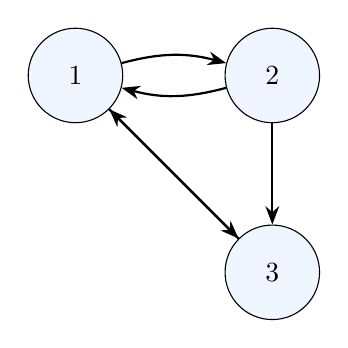
\begin{tikzpicture}[>=Stealth, node distance=2.5cm, main/.style = {draw, circle, fill=LightBlue, minimum size=1.2cm}]
  \node[main] (1) {1};
  \node[main] (2) [right of=1] {2};
  \node[main] (3) [below of=2] {3};
  \draw[->, thick] (1) to [bend left=15] (2);
  \draw[->, thick] (2) to [bend left=15] (1);
  \draw[->, thick] (2) -- (3);
  \draw[->, thick] (3) -- (1);
  \draw[->, thick] (1) -- (3);
\end{tikzpicture}
\end{center}
A user starts at a page and at each step clicks a link uniformly at random.
\begin{enumerate}[label=(\alph*)]
  \item Set up the transition matrix $P$ of this random surfer model.
  \item Is the chain irreducible? Is it aperiodic? Explain.
  \item Calculate the PageRank of each page by solving for the stationary distribution.
\end{enumerate}
\end{problem}

\newpage

% ============================================================
\section{Part 7 \texorpdfstring{---}{--} Deep Problems}
% ============================================================

\begin{deepproblem}[The Ehrenfest Urn stationary distribution]
Let $X_n \in \{0, 1, \dots, N\}$ be the number of balls in urn A in the Ehrenfest Urn model (Part 1).
\begin{enumerate}[label=(\alph*)]
  \item Show that the transition probabilities are:
  \[
    P_{i, i+1} \;=\; 1 - \frac{i}{N}, \qquad P_{i, i-1} \;=\; \frac{i}{N},
  \]
  and $P_{ij} = 0$ otherwise.
  \item We search for a stationary distribution $\boldsymbol{\pi}$ using detailed balance: $\pi_i P_{i, i+1} = \pi_{i+1} P_{i+1, i}$. Write this relation explicitly.
  \item Solve the recurrence relation from (b) to show that:
  \[
    \pi_i \;=\; \binom{N}{i} \pi_0.
  \]
  \item Use the binomial theorem to normalize the distribution, showing that $\pi_0 = 2^{-N}$, and therefore:
  \[
    \pi_i \;=\; \binom{N}{i} 2^{-N}.
  \]
  Explain why this stationary distribution shows that in equilibrium, the balls are distributed according to a binomial distribution. Why does this resolve the reversibility paradox for large $N$ (e.g. $N = 10^{23}$)?
\end{enumerate}
\end{deepproblem}

\begin{deepproblem}[Perron-Frobenius Theorem and Stationarity]
The existence of a stationary distribution depends on the eigenvalue structure of stochastic matrices.
The **Perron-Frobenius Theorem** states that any non-negative irreducible square matrix $A$ has a unique largest positive eigenvalue $r$, and the corresponding eigenvector has strictly positive components.
\begin{enumerate}[label=(\alph*)]
  \item Let $P$ be a stochastic transition matrix. Show that $\mathbf{e} = (1, 1, \dots, 1)^T$ is a right eigenvector of $P$ with eigenvalue 1.
  \item Show that the eigenvalues of $P$ satisfy $|\lambda| \le 1$. \textit{Hint: Use the property that row sums of $P^n$ are 1.}
  \item Use the Perron-Frobenius theorem to prove that any finite, irreducible Markov chain must possess a unique stationary distribution.
\end{enumerate}
\end{deepproblem}

\newpage

% ============================================================
\section{Part 8 \texorpdfstring{---}{--} Reflection}
% ============================================================

\begin{reflectionbox}
\textbf{Conceptual Reflection}

Consider the following questions:
\begin{enumerate}
  \item **On Equilibrium and Irreversibility:** The Ehrenfest model shows that microscopic reversibility is fully compatible with macroscopic convergence to a binomial peak at $N/2$. For $N=10^{23}$, why does the system never return to the state where all particles are in one urn, even though the state is technically recurrent?
  \item **On the Markov Property:** PageRank models web surfing as a Markov chain. But real surfers have history (they press the back button, search history). How would you modify the model to account for memory, and does it remain a Markov chain if we expand the state space?
  \item **On detailed balance:** Detailed balance is a property of physical systems in thermodynamic equilibrium. Why does detailed balance mean that "time-reversed" paths look exactly like forward paths?
\end{enumerate}
\end{reflectionbox}

\medskip
\noindent\textbf{Looking ahead.}
Module~6 completes this journey by introducing **Advanced Bayesian Inference & Stochastic Processes**. We will discover how to model continuous-time processes like radioactive decay (Poisson processes) and the random motion of particles (Brownian motion), and apply Bayesian updating to continuous parameters. Symmetries in probability will meet physical kinetics.

\vspace{1.4cm}
\begin{center}
{\color{MidBlue}\rule{0.5\linewidth}{0.8pt}}\\[6pt]
{\small\color{DarkGrey}\textit{End of Journey 5, Module 5 --- Markov Chains and Transition Matrices}}\\[4pt]
{\small\color{DarkGrey}Continue to: \textbf{Module 6 --- Bayesian Inference and Stochastic Processes}}\\[6pt]
{\color{MidBlue}\rule{0.5\linewidth}{0.8pt}}
\end{center}

\end{document}
